\newcommand{\MHpm}{M_{\PSHpm}}

\section{MSSM charged Higgs production process\footnote{M.~Flechl,
    M.~Kr\"amer, S.~Lehti (eds.); S.~Dittmaier, T.~Hahn, 
    T.~Hartonen, S.~Heinemeyer, J.~S.~Lee, A.~Pilaftsis, 
    M.~Spira and C.~Weydert.}}
\label{sec:chiggs_intro}

Many extensions of the Standard Model, in particular supersymmetric
theories, require two Higgs doublets leading to five physical scalar
Higgs bosons, including two (mass-degenerate) charged particles $\PSHpm$.
The discovery of a charged Higgs boson would provide
unambiguous evidence for an extended Higgs sector beyond the Standard
Model. Searches at LEP have set a limit $\MHpm > 79.3$\UGeV\ 
on the mass of a charged Higgs boson in a general two-Higgs-doublet
model~\cite{Heister:2002ev}. Within the MSSM, the charged Higgs-boson
mass is constrained by the pseudoscalar Higgs mass and the W-boson
mass through $\MHpm^2 = \MA^2 + \MW^2$ at
tree level, with only moderate higher-order
corrections~\cite{Gunion:1988pc, Brignole:1991wp, Diaz:1991ki,
  Frank:2006yh}. A mass limit on the MSSM charged Higgs boson can thus
be derived from the limit on the pseudoscalar Higgs boson, 
$\MA > 93.4$\UGeV~\cite{Schael:2006cr}, resulting in 
$\MHpm \gsim 120$\UGeV. At the Tevatron, searches for light charged
Higgs bosons in top-quark decays $\Pt \to \Pb \PSHpm$~\cite{Aaltonen:2009ke,:2009zh} have placed some constraints
on the MSSM parameter space, but do not provide any further generic
bounds on $\MHpm$.

There are two main mechanisms for charged Higgs-boson production at
the LHC:
\begin{displaymath}
\begin{array}{lcl}
  \mbox{top-quark decay:} & \Pt \to \Pb \PSHpm{\rm + X} &\; {\rm if}\;\;
  \MHpm \lsim m_{\rm t}\,, \\
  \mbox{associated production:} & \Pp\Pp \to \Pt \Pb\PSHpm{\rm + X}
  &\; {\rm if}\;\; \MHpm \gsim \Mt\,.
\end{array}
\end{displaymath}
Alternative production mechanisms like quark--antiquark annihilation
$\Pq\bar \Pq'\to \PSHpm$ and $\PSHpm+\mathrm{jet}$ production~\cite{Dittmaier:2007uw},
associated $\PSHpm \PWmp$ production~\cite{Eriksson:2006yt}, or 
Higgs pair production~\cite{Alves:2005kr,Brein:1999sy} have
suppressed rates, and it is not yet clear whether a signal could be
established in any of those channels. 
Some of the above production processes may,
however, be enhanced in models with non-minimal flavour violation.

In this section we discuss charged Higgs-boson production in $\Pt \to
\Pb \PSHpm$ decays and compare the results of different software
packages for the calculation of this branching ratio. Furthermore, we
present NLO QCD predictions for the process $\Pp\Pp \to \Pt\Pb 
\PSHpm{\rm + X}$ in the four- and five-flavour schemes.

\subsection{Light charged Higgs production from top-quark decays}

If the charged Higgs boson is light, $\MHpm \lsim \Mt$, 
it is produced in top-quark decays. The branching ratio
calculation of the top quark to a light charged Higgs boson is
compared for two different programs, {\sc FeynHiggs}, version
2.7.3~\cite{Heinemeyer:1998yj,Heinemeyer:1998np,Degrassi:2002fi,Frank:2006yh},
and {\sc CPsuperH}, version 2.2~\cite{Lee:2003nta,Lee:2007gn}. 
We note that the decay  $\Pt \to \PSHp \Pb$ is also included in {\sc HDECAY}~\cite{Djouadi:1997yw}, 
which has however not been included in the comparison presented here. 
The
$m_h^{\rm max}$ benchmark scenario was used~\cite{Carena:2002qg},
which in the on-shell scheme is defined as described 
in \Eq~(\ref{YRHXS_MSSM_neutral_eq:mhmax}).
In addition to $\tan \beta$ and $\MHpm$, the $\mu$ parameter
was varied with values $\pm 1000, \pm 200$\UGeV~\cite{Carena:2005ek}. 
The Standard Model parameters were taken as given in the 
Appendix \Table~\ref{tab:SMinput}.

The calculation within {\sc FeynHiggs} is based on the evaluations of
$\Gamma(\Pt \to \PWp \Pb)$ and $\Gamma(\Pt \to \PSHp \Pb)$. The former is
calculated at NLO according to \Bref{Campbell:2004ch}. The decay
to the charged Higgs boson and the bottom quark uses $\Mt(\Mt)$ and 
$\Mb(\Mt)$ in the Yukawa coupling, where the
latter receives the additional correction factor $1/(1 +
\Delta_{\Pb})$. The leading contribution to $\Delta_{\Pb}$ is given
by~\cite{Carena:1999py}
\begin{equation}
\label{eq:qcd_tanb_enhanced}
\Delta_{\Pb} = \frac{C_F}{2}\frac{\alphas}{\pi} 
m_{\tilde{\Pg}} \mu \tan\beta  \,
I(m_{\tilde{\Pb}_1},m_{\tilde{\Pb}_2},m_{\tilde{\Pg}}) \, ,
\end{equation}
with $C_F = 4/3$ and the auxiliary function
\begin{equation}
\label{eq:I}
I(a,b,c) = \frac{1}{(a^2-b^2)(b^2-c^2)(a^2-c^2)} \left(
a^2 b^2 \ln \frac{a^2}{b^2} + 
b^2 c^2 \ln \frac{b^2}{c^2} + 
c^2 a^2 \ln \frac{c^2}{a^2}
\right) \, .
\end{equation}
Here, $\tilde{\Pb}_{1,2}$ are the sbottom mass eigenstates, and
$m_{\tilde{\Pg}}$ is the gluino mass. The numerical results presented
here have been based on the evaluation of $\Delta_{\Pb}$ in
\Bref{Hofer:2009xb}.  
Furthermore additional QCD corrections taken from
\Bref{Carena:1999py} are included.

The calculation within {\sc CPsuperH} is also based on the top-quark
decays $\Pt \to \PWp \Pb$ and $\Pt \to \PSHp \Pb$.  The decay width
$\Gamma(\Pt \to \PWp \Pb)$ is calculated by including ${\cal
  O}(\alphas)$ corrections~\cite{Chetyrkin:1999br}.
%
The partial decay width of the decay $\Pt \to \PSHp \Pb$ is given by
\begin{eqnarray}
\Gamma(\Pt\rightarrow \PH^+ b)&=&\frac{g_{\Pt\Pb}^2\Mt}{16\pi}
\left(|g^S_{_{{\PH}^+\bar{\Pt}{\rm b}}}|^2+|g^P_{_{\PH^+\bar{\Pt}{\rm b}}}|^2\right)
\left(1-\frac{\MHpm^2}{\Mt^2}\right)^2\,,
\end{eqnarray}
where $g_{\Pt\Pb} = - g \Mt/\sqrt{2} \MW$, 
      $g^S_{\PSHp\bar{\Pt}\Pb}=(g^L_{\PSHp\bar{\Pt}\Pb} + 
      \frac{\Mb}{\Mt}\, g^R_{\PSHp\bar{\Pt}\Pb})/2$, 
      and $g^P_{\PSHp\bar{\Pt}\Pb}=i(g^L_{\PSHp\bar{\Pt}\Pb} 
      - \frac{\Mb}{\Mt}\, g^R_{\PSHp\bar{\Pt}\Pb})/2$.  
In the couplings $g^{L,R}_{\PSHp\bar{\Pt}\Pb}$, all the
threshold corrections (both those enhanced and not enhanced by
$\tan\beta$) have been included as described in Appendix A of
\Bref{Lee:2003nta} and \Refs~\cite{Carena:2002bb,Ellis:2009di},
see also \Bref{Guasch:2003cv}. 
%
For $\Mt$ and $\Mb$ appearing in the couplings, we use the
quark masses evaluated at the scale $\MHpm$.

The comparison started by running {\sc FeynHiggs} with a selected set
of parameters. The {\sc FeynHiggs} output was used to set the values
for the CPsuperH input parameters. Due to differences in the parameter
definitions, the bottom-quark mass was changed from {\sc FeynHiggs}
$\Mb(\Mb) = 4.16$\UGeV\ to $\Mb(\Mt) = 2.64$\UGeV\ 
which is taken as input by {\sc CPsuperH}. The main result
from the comparison is shown in Figs.~\ref{fig:BRTop2HPlus} and
\ref{fig:BRTop2HPlusDiff}. A very good agreement within typically $0{-}2\%$ 
can be observed, except if simultaneously very small values of $\mu$, 
high $\tan\beta$, and relatively small $\MHpm$ are chosen.

\begin{figure}[ht]
  \centering
\begin{tabular}{cc}
  \includegraphics[width=0.46\textwidth]{YRHXS_MSSM_charged/YRHXS_MSSM_charged_fig1a.eps} &
  \includegraphics[width=0.46\textwidth]{YRHXS_MSSM_charged/YRHXS_MSSM_charged_fig1b.eps} \\
  \includegraphics[width=0.46\textwidth]{YRHXS_MSSM_charged/YRHXS_MSSM_charged_fig1c.eps} &
  \includegraphics[width=0.46\textwidth]{YRHXS_MSSM_charged/YRHXS_MSSM_charged_fig1d.eps} \\  
\end{tabular}
\caption{The branching fraction of $\Pt\rightarrow \Pb\PSHpm$ as a
  function of $\tan\beta$ for different values of $\mu$ and $\MHpm$. 
  The lines in the upper left plot terminate when the specific code
  reaches a negative light Higgs mass squared. Depending on the code this
  happens for slightly smaller or larger $\tan\beta$ values (in this
  extreme scenario).
%  The solid black curves are calculated with {\sc FeynHiggs}, 
%  and the dotted green curves with {\sc CPsuperH}.
}
\label{fig:BRTop2HPlus}
\end{figure}

\begin{figure}[ht]
  \centering
   \begin{tabular}{cc}
   \includegraphics[width=0.46\textwidth]{YRHXS_MSSM_charged/YRHXS_MSSM_charged_fig2a.eps} &
   \includegraphics[width=0.46\textwidth]{YRHXS_MSSM_charged/YRHXS_MSSM_charged_fig2b.eps} \\
   \includegraphics[width=0.46\textwidth]{YRHXS_MSSM_charged/YRHXS_MSSM_charged_fig2c.eps} &
   \includegraphics[width=0.46\textwidth]{YRHXS_MSSM_charged/YRHXS_MSSM_charged_fig2d.eps} \\
  \end{tabular}
\caption{The difference of BR($\Pt\rightarrow \Pb\PSHpm$) calculated
  with {\sc CPsuperH} and {\sc FeynHiggs} as a function of $\tan\beta$
  for different values of $\mu$ and $\MHpm$.}
\label{fig:BRTop2HPlusDiff}
\end{figure}

\subsection{Heavy charged Higgs production with top and bottom quarks}
\label{subsec:CH_tbh}

For heavy charged Higgs bosons,  $\MHpm \gsim \Mt$,
associated production $\Pp\Pp \to {\Pt}\Pb \PSHpm{\rm + X}$ is the
dominant production mode. 
Two different formalisms can be employed to calculate the cross
section for associated ${\Pt}\Pb\PSHpm$ production.  In the
four-flavour scheme (4FS) with no $\Pb$ quarks in the initial state,
the lowest-order QCD production processes are gluon--gluon fusion and
quark--antiquark annihilation, $\Pg\Pg \to {\Pt}\Pb\PSHpm$ and
$\Pq\bar \Pq \to {\Pt}\Pb\PSHpm$, respectively. Potentially
large logarithms $\propto \ln(\mu_{\rm F}/\Mb)$, which arise from
the splitting of incoming gluons into nearly collinear $\Pb\bar \Pb$
pairs, can be summed to all orders in perturbation theory by
introducing bottom parton densities. This defines the five-flavour
scheme (5FS)~\cite{Barnett:1987jw}. The use of bottom distribution
functions is based on the approximation that the outgoing $\Pb$ quark
is at small transverse momentum and massless, and the virtual $\Pb$
quark is quasi on shell. In this scheme, the leading-order (LO)
process for the inclusive $\Pt\Pb\PSHpm$ cross section is
gluon--bottom fusion, $\Pg \Pb \to \Pt \PSHpm$.  The next-to-leading
order (NLO) cross section in the 5FS includes ${\cal
  O}(\alphas)$ corrections to $\Pg \Pb \to \Pt  \PSHpm$
and the tree-level processes $\Pg\Pg \to \Pt\Pb\PSHpm$ and $\Pq\bar
\Pq \to \Pt\Pb\PSHpm$. To all orders in perturbation theory the four-
and five-flavour schemes are identical, but the way of ordering the
perturbative expansion is different, and the results do not match
exactly at finite order. For the inclusive production of neutral Higgs 
bosons with bottom quarks, $\Pp\Pp \to \Pb\bar{\Pb}\PH{\rm + X}$, the
four- and five-flavour scheme calculations numerically agree within
their respective uncertainties, once higher-order QCD corrections are
taken into account~\cite{Dittmaier:2003ej, Campbell:2004pu,
  Dawson:2005vi, Buttar:2006zd}, see \Section~6 of this Report.
  
There has been considerable progress recently in improving the cross-section 
predictions for the associated production of charged Higgs
bosons with heavy quarks by calculating NLO SUSY QCD and electroweak
corrections in the four- and five-flavour schemes~\cite{Zhu:2001nt,
  Gao:2002is, Plehn:2002vy, Berger:2003sm, Kidonakis:2005hc,
  Peng:2006wv, Beccaria:2009my, Kidonakis:2010ux}, and the matching of
the NLO five-flavour scheme calculation with parton
showers~\cite{Weydert:2009vr}. Below, we shall present
state-of-the-art NLO QCD predictions in the 4FS
(\Section~\ref{subsubsec:CH_4FS}), in the 5FS
(\Section~\ref{subsubsec:CH_5FS}), and a first comparison of the two
schemes at NLO (\Section~\ref{subsubsec:CH_4and5FS}).

\subsubsection{NLO QCD predictions for $\Pp\Pp \to \Pt\Pb\PSHpm$ in the 4FS}
\label{subsubsec:CH_4FS}

In the 4FS the production of charged Higgs bosons in association with
top and bottom quarks proceeds at LO through the parton processes
$\Pg\Pg \to {\Pt}\bar{\Pb}\PSHm$ and $\Pq\bar{\Pq} \to \Pt\bar{\Pb}\PSHm$, 
and the charge-conjugate processes with the
$\bar{\Pt}\Pb\PSHp$ final state~\cite{DiazCruz:1992gg,
  Borzumati:1999th, Miller:1999bm}. Throughout this section we present
results for the ${\Pt}\bar{\Pb} \PSHm$ channels. Generic Feynman
diagrams that contribute at LO are displayed in \Fref{fig:diags}.
\begin{figure}
\begin{center}
%\epsfig{file=YRHXS_MSSM_charged/feyn.ps,%
%%  bbllx=55pt,bblly=625pt,bburx=596pt,bbury=842pt,%
%  bbllx=55pt,bblly=625pt,bburx=446pt,bbury=842pt,%
%        clip=,scale=0.8}
\SetScale{0.8}
\begin{picture}(130,90)(0,0)
\ArrowLine(0,100)(50,50)
\ArrowLine(50,50)(0,0)
\Gluon(50,50)(100,50){3}{5}
\ArrowLine(100,50)(120,70)
\ArrowLine(120,70)(150,100)
\ArrowLine(150,0)(100,50)
\DashLine(120,70)(150,70){5}
\Vertex(50,50){2}
\Vertex(100,50){2}
\Vertex(120,70){2}
\put(-12,78){$\PQq$}
\put(-12,-2){$\PAQq$}
\put(125,53){$\PH^-$}
\put(125,78){$\PQt$}
\put(125,-2){$\PAQb$}
\end{picture}
\begin{picture}(130,90)(-80,0)
\Gluon(0,0)(50,0){3}{5}
\Gluon(0,100)(50,100){3}{5}
\ArrowLine(100,0)(50,0)
\ArrowLine(50,0)(50,50)
\ArrowLine(50,50)(50,100)
\ArrowLine(50,100)(100,100)
\DashLine(50,50)(100,50){5}
\Vertex(50,100){2}
\Vertex(50,50){2}
\Vertex(50,0){2}
\put(85,35){$\PH^-$}
\put(-12,78){$\Pg$}
\put(-12,-2){$\Pg$}
\put(85,78){$\PQt$}
\put(85,-2){$\PAQb$}
\end{picture}
\vspace*{1em}
\caption{Generic Feynman diagrams for 
          $\Pp\Pp \to {\Pt}\bar\Pb\PSHm{\rm + X}$ in the 4FS at LO.}
\label{fig:diags}
\end{center}
\end{figure}
% ---------------------------------------------------------------------

The calculation of the NLO QCD corrections to charged Higgs production
in the 4FS has been discussed in detail in
\Bref{Dittmaier:2009np}, both within a two-Higgs-doublet model
with the SM particle content besides the extended Higgs sector, and
within the MSSM. The NLO QCD effects considerably enhance the cross
section and reduce the dependence on the renormalization and
factorization scales. In the MSSM, additional loop corrections from
squark and gluino exchange are sizable for large $\tan\beta$, but they
can be taken into account through the $\Delta_{\Pb}$ corrections
to
the bottom--Higgs-Yukawa coupling [cf.\ \Eq~(\ref{eq:qcd_tanb_enhanced})], i.e.\ through a rescaling of
the NLO QCD prediction according to $\Mb\tan\beta/v \to \Mb\tan\beta/v
\, (1 - \Delta_{\Pb}/\tan^2\beta) / (1 +
\Delta_{\Pb})$~\cite{Dittmaier:2009np}.

In \Tables~\ref{tab::charged_higgs_4fs_nlo_7tev} and
\ref{tab::charged_higgs_4fs_nlo_14tev} we present 4FS NLO QCD results
for the production of heavy charged Higgs bosons in a
two-Higgs-doublet model. Cross sections for MSSM scenarios with large
$\tan\beta$ can be obtained from the NLO QCD cross sections by the
rescaling defined above. Predictions are presented for LHC cross
sections at $7\UTeV$ and $14$\UTeV\ energy, with $\tan\beta = 30$ and the SM
input parameters according to \Table~\ref{tab:SMinput}.
%
\begin{table}[h!]
  \caption{\label{tab::charged_higgs_4fs_nlo_7tev}  
    NLO QCD cross sections for 
    $\Pp\Pp \to \Pt\bar{\Pb}\PSHm$ in the 4FS at the LHC with $7$\UTeV, $\tan \beta=30$.}
\centering
%\begin{tabular}{ccccc}\hline
%$\MHpm$~[GeV] & $\sigma$~[\UfbZ] & scale uncert. [\%] & PDF + \alphas\; [\%] & total [\%] \\
%\hline
%$200$ & $130$  &  $-33 \; +27$  & $-5.5 \; +4.5$ & $-33 \; +27$\\
%$300$ & $45.9$ &  $-33 \; +34$  & $-6.7 \; +5.6$ & $-34 \; +34$\\
%$400$ & $18.0$ &  $-34 \; +30$  & $-7.7 \; +6.6$ & $-35 \; +31$\\
%$500$ & $7.59$ &  $-35 \; +32$  & $-8.6 \; +7.5$ & $-36 \; +33$\\
%\hline
%\end{tabular}
\small
\begin{tabular}{crcc}\hline
$\MHpm$~[GeV] & $\sigma$~[\UfbZ] & Scale uncert. [\%] & PDF + \alphas\; [\%]  \\
\hline
$200$ & $130$  &  $-33 \; +27$  & $-5.5 \; +4.5$ \\
$300$ & $45.9$ &  $-33 \; +34$  & $-6.7 \; +5.6$ \\
$400$ & $18.0$ &  $-34 \; +30$  & $-7.7 \; +6.6$ \\
$500$ & $7.59$ &  $-35 \; +32$  & $-8.6 \; +7.5$ \\
\hline
\end{tabular}
\end{table}
%
%\begin{table}[h!]
%  \caption{\label{tab::charged_higgs_4fs_nlo_14tev}  
%    NLO QCD cross sections for 
%    $\Pp\Pp \to \Pt\bar{\Pb}\PSHm$ in the 4FS at the LHC with $14$\UTeV, $\tan \beta=30$.}
%\centering
%\begin{tabular}{ccccc}\hline
%$\MHpm$~[GeV] & $\sigma$~[\UfbZ] & scale uncert. [\%] & PDF + \alphas\; [\%] & total [\%] \\
%\hline
%$200$ & $972$  &  $-30 \; +27$  & $-3.4 \; +2.7$ & $-30 \; +27$\\
%$300$ & $405$  &  $-30 \; +26$  & $-4.0 \; +3.2$ & $-30 \; +26$\\
%$400$ & $184$  &  $-30 \; +26$  & $-4.7 \; +3.7$ & $-30 \; +26$\\
%$500$ & $92.6$ &  $-32 \; +29$  & $-5.1 \; +4.1$ & $-32 \; +29$\\
%\hline
%\end{tabular}
\begin{table}[h!]
  \caption{\label{tab::charged_higgs_4fs_nlo_14tev}  
    NLO QCD cross sections for 
    $\Pp\Pp \to \Pt\bar{\Pb}\PSHm$ in the 4FS at the LHC with $14$\UTeV, $\tan \beta=30$.}
\centering
\small
\begin{tabular}{crcc}\hline
$\MHpm$~[GeV] & $\sigma$~[\UfbZ] & Scale uncert. [\%] & PDF + \alphas\; [\%] \\
\hline
$200$ & $972$  &  $-30 \; +27$  & $-3.4 \; +2.7$ \\
$300$ & $405$  &  $-30 \; +26$  & $-4.0 \; +3.2$ \\
$400$ & $184$  &  $-30 \; +26$  & $-4.7 \; +3.7$ \\
$500$ & $92.6$ &  $-32 \; +29$  & $-5.1 \; +4.1$ \\
\hline
\end{tabular}
\end{table}

For a consistent evaluation of the hadronic cross sections in the 4FS
we adopt the recent MSTW four-flavour PDF~\cite{Martin:2010db} and the
corresponding four-flavour $\alphas$.  Note, however, that the
evaluation of the running \Pb-quark mass in the bottom--Higgs-Yukawa
coupling is based on a five-flavour $\alphas$ with 
$\alphas(\MZ) = 0.120$. The renormalization and factorization scales have
been identified and are set to $\mu = (\Mt + \Mb + M_{\PSHm})/3$ 
as our default choice. The NLO scale uncertainty has
been estimated from the variation of the renormalization and
factorization scales by a factor of three about the central scale
choice $\mu = (\Mt + \Mb + M_{\PSHm})/3$. As shown in \Bref{Dittmaier:2009np}, the variation of
the QCD scales by a factor three about the central scale provides
a more reliable estimate of the theory uncertainty than the usual
variation by a factor two, as the variation by a factor three encompasses 
the maximum of the NLO prediction. The residual NLO scale
uncertainty is then approximately $\pm 30$\%. While no four-flavour PDF
parametrization exists that would allow to estimate the combined PDF
and $\alphas$ error, the difference in the relative PDF error
as obtained from the MSTW four- and five-flavour sets is marginal.  We
have thus adopted the five-flavour MSTW PDF~\cite{Martin:2009iq} to
estimate the combined PDF and $\alphas$ uncertainty shown in
\Tables~\ref{tab::charged_higgs_4fs_nlo_7tev} and
\ref{tab::charged_higgs_4fs_nlo_14tev}. We find that the theoretical
uncertainty of the 4FS NLO QCD prediction for 
$\Pp\Pp \to \Pt \bar{\Pb}\PSHm$ at the LHC is by far 
dominated by the scale uncertainty.

The NLO QCD cross section for 
$\Pp\Pp \to {\Pt}\bar{\Pb}\PSHm$ at the LHC with $7\UTeV$ and $14$\UTeV\ is shown in
\Fref{fig:totalxs} as a function of the Higgs-boson mass. The
%error band includes the NLO scale uncertainty and the 
%PDF+$\alphas$ error, added in quadrature.
error band quantify the NLO scale uncertainty.

%%%%%%%%%%%%%%%%%%%%%%%%%%%%%%%%%%%%%

\begin{figure}
\begin{center}
% \includegraphics[bb = 170 530 500 820, %width=0.48\textwidth]{YRHXS_MSSM_charged/totalxs_7TeV.eps}
% \includegraphics[bb = 170 530 500 820, %width=0.48\textwidth]{YRHXS_MSSM_charged/totalxs_14TeV.eps}
\includegraphics[width=0.48\textwidth]{YRHXS_MSSM_charged/YRHXS_MSSM_charged_fig4a.eps}
\includegraphics[width=0.48\textwidth]{YRHXS_MSSM_charged/YRHXS_MSSM_charged_fig4b.eps}

 \caption{NLO QCD cross sections for 
     $\Pp\Pp \to {\Pt}\bar{\Pb}\PSHm$ in the 4FS at the LHC ($7$\UTeV\ and $14$\UTeV) as a function of
   the Higgs-boson mass. The error band includes the NLO scale
   uncertainty. 
   (Calculation from \Bref{Dittmaier:2009np}.)}
\label{fig:totalxs}
\end{center}
\end{figure}
        
%%%%%%%%%%%%%%%%%%%%%%%%%%%%%%%%%%%%%

\subsubsection{NLO QCD predictions for $\Pp\Pp \to \Pt \PSHpm$ in the 5FS}
\label{subsubsec:CH_5FS}

In the 5FS the LO process for the inclusive $\PSHpm$ cross
section is gluon--bottom fusion, $\Pg \Pb \to \Pt \PSHpm$. The NLO
cross section includes ${\cal O}(\alphas)$ corrections to
$\Pg \Pb \to \Pt \PSHpm$ and the tree-level processes $\Pg\Pg \to
\Pt\Pb\PSHpm$ and $\Pq\bar \Pq \to \Pt\Pb\PSHpm$, and has been
calculated in \Refs~\cite{Plehn:2002vy, Berger:2003sm,
  Weydert:2009vr}. In \Tables~\ref{tab::charged_higgs_5fs_nlo_7tev}
and \ref{tab::charged_higgs_5fs_nlo_14tev} we present NLO QCD results
for the production of heavy charged Higgs bosons in the 5FS, with
$\tan\beta = 30$ and the SM input parameters according to
\Table~\ref{tab:SMinput}. As in the 4FS calculation, cross sections
for MSSM scenarios with large $\tan\beta$ can be obtained from the
NLO QCD cross sections by rescaling the bottom--Higgs-Yukawa coupling.
%
\begin{table}[h!]
  \caption{\label{tab::charged_higgs_5fs_nlo_7tev}  
    NLO QCD cross sections for 
    $\Pp\Pp \to \Pt\PSHm$ in the 5FS at the LHC with $7$\UTeV, $\tan \beta=30$.}
  \centering
  \small
  \begin{tabular}{crr}\hline
$\MHpm$~[GeV] & $\sigma$~[\UfbZ] & Scale uncert. [\%] \\
\hline
$200$ & $178$  &  $-7.1  \; +9.4$~~  \\
$300$ & $62.7$ &  $-10.0 \; +4.7$~~  \\
$400$ & $24.7$ &  $-11.0 \; +2.7$~~  \\
$500$ & $10.5$ &  $-12.0 \; +1.1$~~  \\
\hline
\end{tabular}
\end{table}
%
\begin{table}[h!]
  \caption{\label{tab::charged_higgs_5fs_nlo_14tev}  
    NLO QCD cross sections for 
    $\Pp\Pp \to \Pt\PSHm$ in the 5FS at the LHC with $14$\UTeV, $\tan \beta=30$.}
\centering
\small
\begin{tabular}{crr}\hline
$\MHpm$~[GeV] & $\sigma$~[\UfbZ] & Scale uncert. [\%] \\
\hline
$200$ & $1237$ &  $-8.4  \; +13$\phantom{.}~~  \\
$300$ & $521$  &  $-9.0  \; +9.5$~~  \\
$400$ & $242$  &  $-9.8  \; +7.7$~~  \\
$500$ & $121$  &  $-10.0 \; +6.5$~~ \\
\hline
\end{tabular}
\end{table}
The NLO cross section values have been obtained using 
{\sc MC@NLO 4.0}~\cite{Frixione:2010wd}, with the option {\tt rflag} switched to 0 (for MSbar
Yukawa renormalization). The central scale has been set to
$\mu_0=(\Mt+M_{\PSHm})/4$, and the five-flavour MSTW
PDF~\cite{Martin:2009iq} has been adopted. We find a residual NLO
scale uncertainty of $10{-}20\%$. Since there are no direct experimental
constraints on the bottom PDF, the PDF uncertainty of the $\Pg \Pb \to
\Pt \PSHpm$ process is difficult to quantify. Thus, unfortunately,
no reliable estimates of the PDF and $\alphas$ uncertainty of
the 5FS calculation exist to date.

The total 5FS NLO QCD cross section for 
$\Pp\Pp \to \Pt\PSHm$ at the LHC with $7\UTeV$ and $14$\UTeV\ 
is shown in
\Fref{fig:totalxs_5fs} as a function of the Higgs-boson mass.
The error band includes the NLO scale uncertainty only.

\begin{figure}
\begin{center}
%\includegraphics[width=0.48\textwidth]{YRHXS_MSSM_charged/xs7TeV_5fs.eps}
%\includegraphics[width=0.48\textwidth]{YRHXS_MSSM_charged/xs14TeV_5fs.eps}
\includegraphics[width=0.48\textwidth]{YRHXS_MSSM_charged/YRHXS_MSSM_charged_fig5a.eps}
\includegraphics[width=0.48\textwidth]{YRHXS_MSSM_charged/YRHXS_MSSM_charged_fig5b.eps}
\caption{NLO QCD cross sections for $\Pp\Pp \to {\Pt}\PSHm$ in the 5FS at the LHC ($7$\UTeV\ and $14$\UTeV) as a function of
  the Higgs-boson mass. The error band includes the NLO scale
  uncertainty. (Calculation from \Bref{Weydert:2009vr}.)}
\label{fig:totalxs_5fs}
\end{center}
\end{figure}
        
Note that supersymmetric electroweak ${\cal O(\alpha)}$ corrections to
charged Higgs-boson production in the five-flavour scheme have been
studied in \Bref{Beccaria:2009my}. These corrections depend
sensitively on the MSSM scenario and have thus not been included in
the numbers presented here.

\subsubsection{Comparison of the 4FS and 5FS calculations}
\label{subsubsec:CH_4and5FS}

The 4FS and 5FS calculations represent different ways of ordering the
perturbative expansion, and the results will not match exactly at
finite order. However, taking into account higher-order corrections,
the two predictions are expected to agree within their respective
uncertainties, see \Section~\ref{sec:mssm_neutral} of this Report for a similar comparison
for the inclusive production of neutral Higgs bosons with bottom
quarks.

In \Fref{fig:4fs_5fs} we present a comparison of the 4FS and
5FS calculations at NLO QCD for the inclusive 
$\Pp \Pp \to \Pt  \PSHm(\bar{\Pb})$ cross section at the LHC.
%
\begin{figure}
\begin{center}
\includegraphics[width=0.48\textwidth]{YRHXS_MSSM_charged/YRHXS_MSSM_charged_fig6a.eps}
\includegraphics[width=0.48\textwidth]{YRHXS_MSSM_charged/YRHXS_MSSM_charged_fig6b.eps}
%\includegraphics[bb = 170 530 500 820, %width=0.48\textwidth]{YRHXS_MSSM_charged/totalxs_7TeV_4vs5FS.eps}
%\includegraphics[bb = 170 530 500 820, %width=0.48\textwidth]{YRHXS_MSSM_charged/totalxs_14TeV_4vs5FS.eps}
\caption{NLO QCD cross sections for 
    $\Pp\Pp \to {\Pt}\PSHm(\bar{\Pb})$ in the 4FS and 5FS at the LHC 
($7$\UTeV\ and $14$\UTeV) as a
  function of the Higgs-boson mass. The error band includes the NLO
  scale uncertainty. (Calculations from \Refs~\cite{Dittmaier:2009np,
    Weydert:2009vr}.)}
\label{fig:4fs_5fs}
\end{center}
\end{figure}
%        
The error band indicates the theoretical uncertainty when the
renormalization and factorization scales are varied between $\mu_0/3$
and $3\mu_0$,  with  $\mu_0 = (\Mt + \Mb + M_{\PSHm})/3$ 
and $\mu_0=(\Mt+M_{\PSHm})/4$ for the 4FS and 5FS 
calculations, respectively. 
Taking the scale uncertainty into account, the 4FS and
5FS cross sections at NLO are consistent, even though the predictions
in the 5FS at our choice of the central scales are larger than those of
the 4FS by approximately $30\%$, almost independently of the Higgs-boson
mass. Qualitatively similar results have been obtained from a
comparison of 4FS and 5FS NLO calculations for single-top production
at the LHC~\cite{Campbell:2009ss}. Note that the bottom PDF of the
recent five-flavour MSTW fit~\cite{Martin:2009iq} is considerably
smaller than that of previous fits~\cite{Martin:2004ir} and has lead
to a significant decrease in the 5FS cross section prediction.

%\section*{Acknowledgments}
%This work is supported in part by the European Community's Marie-Curie
%Research Training Network under contract MRTN-CT-2006-035505 ``Tools
%and Precision Calculations for Physics Discoveries at Colliders'', the
%DFG SFB/TR9 ``Computational Particle Physics'', and the Helmholtz
%Alliance ``Physics at the Terascale''.

\clearpage
